%----------------------------------------------------------------------
%  Front matter
%----------------------------------------------------------------------
\begin{titlepage}
\centering
\vspace*{1.0cm}

{\large \textsc{International University of Applied Sciences}}\\[0.3cm]


{\LARGE\bfseries Frequent Batch Auction Engine}\\[0.6cm]
{\Large A Design Analysis and Simulation-Based Comparison\\ against Continuous Trading}\\[2.5cm]

{\large Bachelor Thesis}\\[0.4cm]
{\normalsize submitted for the degree of Bachelor of Science}\\[2.5cm]

\begin{figure}
    \centering
    
\includegraphics[width=0.5\linewidth]{Screenshot 2026-09-05 124118.png}
\end{figure}


\begin{tabular}{rl}
\textbf{Author:} & Alejandro Moral Aranda\\
\textbf{Matriculation number:} & 92132071\\
\textbf{Programme:} & B.Sc.\ Data Science\\
\textbf{Supervisor:} & Prof.\ Dr.\ rer.\ nat.\ Hartwig Mayer\\
\textbf{Submission date:} & \today\\
\end{tabular}

\vfill
\end{titlepage}

%----------------------------------------------------------------------
\chapter*{Abstract}
\addcontentsline{toc}{chapter}{Abstract}
\markboth{Abstract}{Abstract}

Continuous limit order books process orders serially, in the sequence in
which they arrive. This single architectural property creates a
mechanical incentive to compete on speed rather than on price, and the
resulting latency arms race imposes a measurable cost on liquidity
demanders. The frequent batch auction (FBA) has been proposed as a
market design response: orders are collected over a short discrete
interval and cleared simultaneously at a single uniform price, so that
being faster within the interval no longer buys a better price.

This thesis studies the FBA from two directions. The theoretical part
decomposes an FBA matching engine into five design blocks: the batch
interval, the information disclosure regime, order flow segregation, the
clearing and rationing rule, and settlement and residual handling. For
each block it sets out the available options and derives, from auction
theory and market microstructure theory, the strategic behaviour each
option induces. The analysis shows that batching does not by itself make
speed worthless. Price-time rationing inside a batch still rewards being
early, and the price improvement that uniform clearing produces is a
transfer between buyers and sellers rather than a gain. When the close of
a batch is predictable, the trader who submits last can steer that
transfer, so the race to be first becomes a race to be last.

The empirical part implements a continuous double auction and a frequent
batch auction with one-second batches, and replays through both the same
order-by-order data of the Solana (SOL) perpetual futures contract on the
Hyperliquid exchange for December 2025. Because both engines receive
identical orders and are compared second by second, any difference
between them comes from the matching mechanism alone.

The main finding is that, at one second, batching largely reproduces the
continuous market with a short delay, and where the two differ the
continuous market comes out slightly ahead. Price formation does not
differ: both engines trade statistically indistinguishable volumes at
closely matching prices, and the same net order flow moves both prices by
the same amount within five seconds. The continuous market is slightly
more liquid, a few percent deeper near the price, and slightly less
volatile, and it executes orders faster: in the batch market orders wait
\ResTimeToExecDiff\,s longer for their first fill. Batching is meant to
add liquidity by gathering buy and sell orders that arrive at different
moments into one auction. In this market, however, trades occur in only
about a quarter of all seconds, so a one-second batch usually contains
just the few orders that would have traded at once in the continuous
market, and there is nothing extra to combine. In the continuous market, resting orders pay a
systematic adverse-selection cost; whether batching lowers it cannot be
measured in the replay, because trades in a batch auction have no
direction. These results describe the mechanical
effect of batching on fixed historical orders, not how traders would
adapt to it.

\vspace{0.6em}
\noindent\textbf{Keywords:} market microstructure; frequent batch
auction; matching engine; latency arbitrage; uniform-price clearing;
Level~4 order book data.

%----------------------------------------------------------------------
\markboth{Declaration of Authenticity}{Declaration of Authenticity}

\includepdf[
  pages=-,
  addtotoc={1,chapter,0,{Declaration of Authenticity},declaration-of-authenticity}
]{attachments/DECLARATION OF AUTHENTICITY.pdf}

\markboth{Grant of Usage Rights}{Grant of Usage Rights}
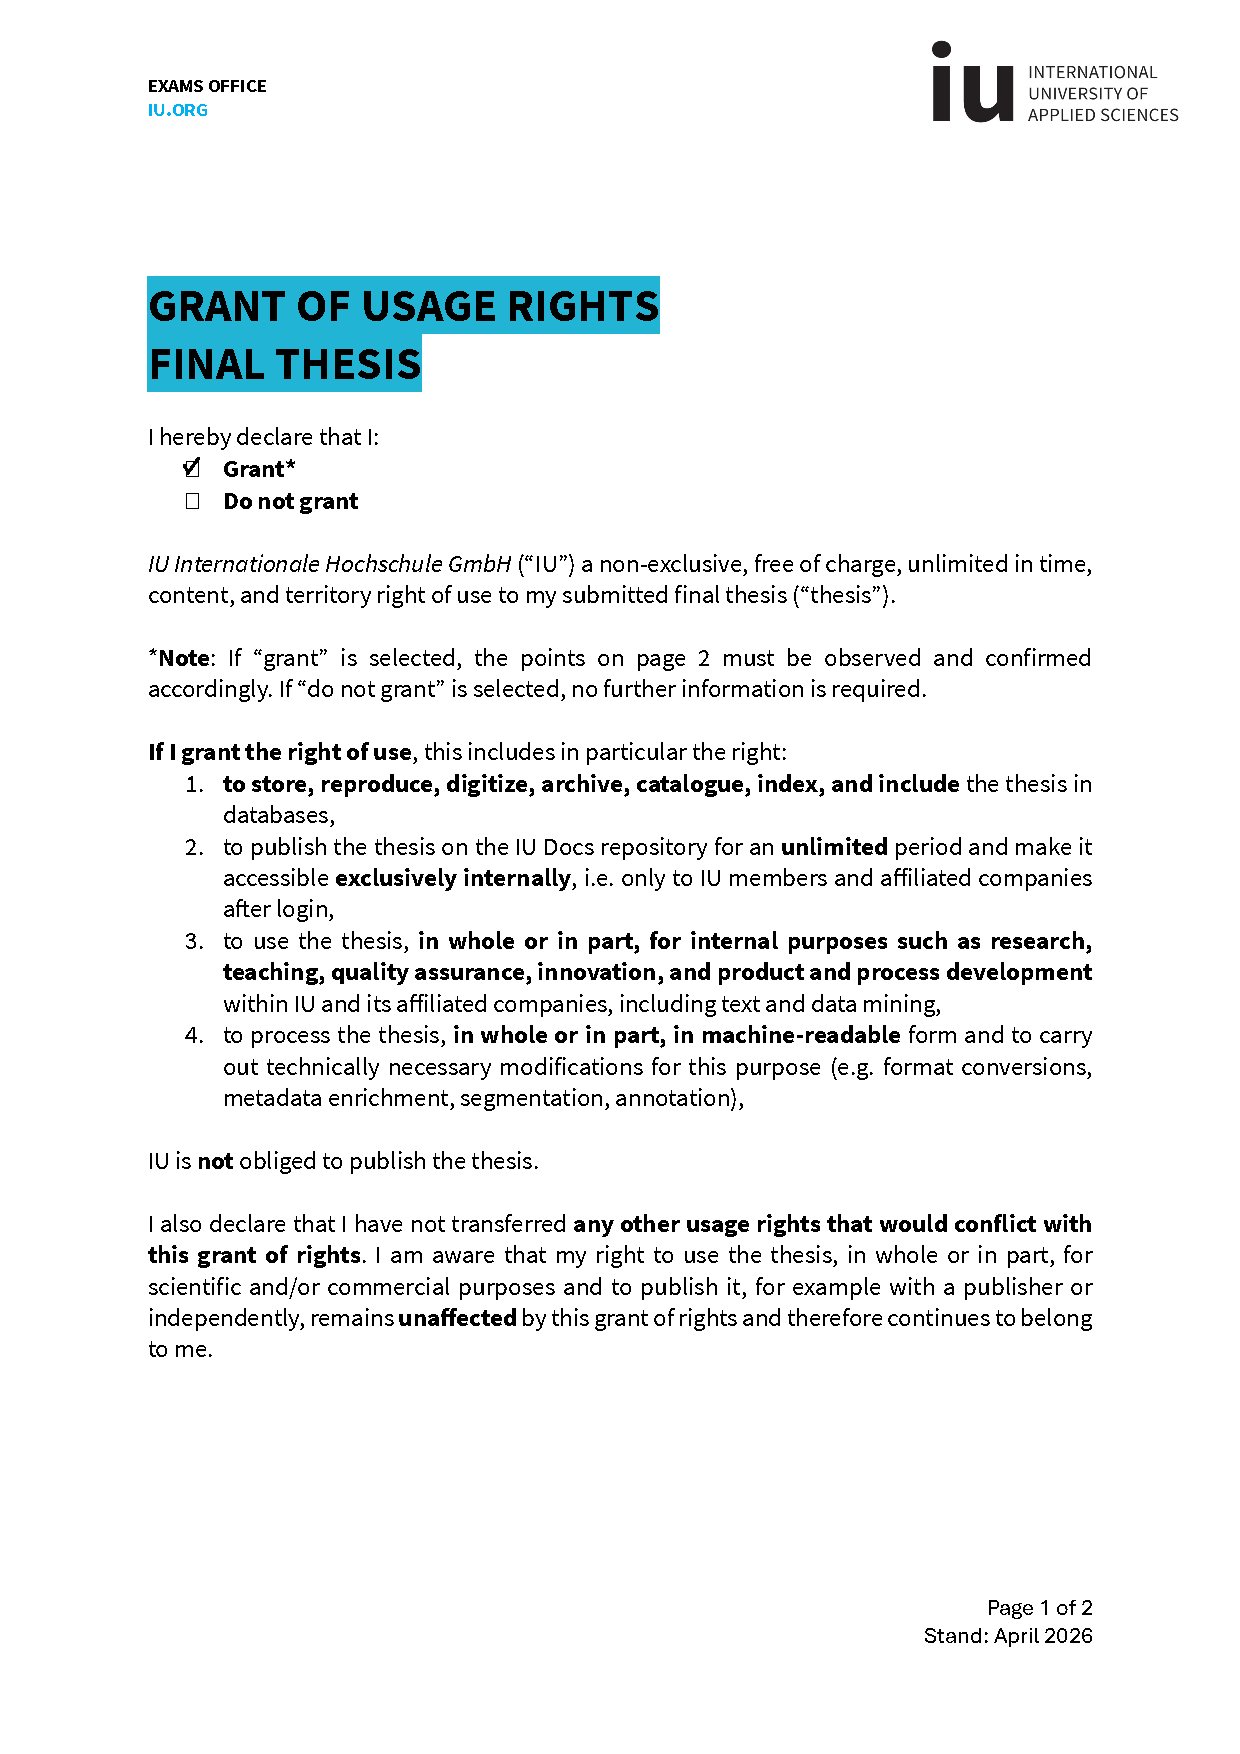
\includepdf[
  pages=-,
  addtotoc={1,chapter,0,{Grant of Usage Rights},grant-of-usage-rights}
]{attachments/Grant of Usage Rights - Thesis_signed.pdf}

%----------------------------------------------------------------------
\cleardoublepage
\setcounter{tocdepth}{1}
\tableofcontents
\cleardoublepage
\addcontentsline{toc}{chapter}{List of Figures}
\listoffigures
\cleardoublepage
\addcontentsline{toc}{chapter}{List of Tables}
\listoftables

%----------------------------------------------------------------------
\cleardoublepage
\chapter*{List of Abbreviations}
\addcontentsline{toc}{chapter}{List of Abbreviations}
\markboth{List of Abbreviations}{List of Abbreviations}

\begin{tabular}{ll}
\toprule
bps   & Basis points ($10^{-4}$)\\
CDA   & Continuous Double Auction\\
CME   & Chicago Mercantile Exchange\\
DFBA  & Dual Flow Batch Auction\\
FBA   & Frequent Batch Auction\\
HAC   & Heteroskedasticity- and Autocorrelation-Consistent (standard errors)\\
IOC   & Immediate-or-Cancel\\
RMS   & Root Mean Square\\
RQ    & Research Question\\
SOL   & Solana (token)\\
USD   & United States Dollar\\
VWAP  & Volume-Weighted Average Price\\
\bottomrule
\end{tabular}
